\subsection{Неветвящиеся трофические цепи}
<<Ресурс>> в реальных экосистемах можно разделить на два вида:
\begin{itemize}
    \item Энергия, например, солнечный свет. Тогда экосистема с данным ресурсом является незамкнутой, и энергия <<протекает>> через систему, в ходе этого рассеиваясь в виде тепла.
    \item Биологические вещества, например, углерод, азот, фосфор. В этом случае экосистема является замкнутой по отношению к ресурсам. Достигается это деятельностью так называемых <<разлагателей>>, которые разлагают мёртвую органику до необходимых минеральных компонентов, необходимых первичным уровням трофической цепи.
\end{itemize}

Соответственно будем рассматривать два типа трофической цепей: незамкнутые (<<проточные>>) и замкнутые (<<циклы>>). Схематически оба эти типа изображены на рис. \ref{shemas}.

Рост и развитие экосистем во многих системах лимитируется каким-либо фактором (\textit{принцип Либиха}). Опять же, например, солнечный свет -- это невозобновимый ресурс и цепь является незамкнутой, а химические вещества за счёт разлагателей снова вовлекаются в деятельность замкнутой экосистемы.

Рассмотрим подробнее схемы на рис. \ref{shemas}. Здесь \(R\) -- ресурс, используемый \(1\)-м видом с биомассой \(N_1\). Удельная скорость использования \(V_0(R)\) -- это количество ресурса, потребляемое единицей биомассы (одной особью) \(1\)-го вида за единицу времени. Из общего количества потребляемого ресурса \(V_0(R)\) только \(k_1\)-доля его идёт на воспроизводство новой биомассы первого вида, остальное расходуется на поддержание жизнедеятельности. Кроме того, с постоянной скоростью \(m_1\) биомасса \(1\)-го вида отмирает. Далее, \(2\)-й вид использует уже в качестве ресурса биомассу \(1\)-го вида, потребляя её с удельной скоростью \(V_1(N_1)\), и т.д. Цепочка заканчивается на \(n\)-м виде, биомассу которого уже никто не потребляет, и он только отмирает со скоростью \(m_n\).

\begin{figure}[H]
\centering
\begin{tikzpicture}

    \usetikzlibrary{shapes.geometric, calc}

    \tikzstyle{roundnode} = [draw, circle, text centered];
    \tikzstyle{squarenode} = [draw, regular polygon, regular polygon sides=4, text centered, inner sep=0];
    \tikzstyle{arrow} = [thick, ->, >=stealth];

    % Left - Flow
    \node[roundnode] (RF) at (0,8) {$R$};

    \node[squarenode] (NF1) at (0,6) {$N_1$};
    \node (NF1M) at (2,6) {$m_1 N_1$};
    \draw [arrow] (NF1) -- (NF1M);

    \node[squarenode] (NF2) at (0,4) {$N_2$};
    \node (NF2M) at (2,4) {$m_2 N_2$};
    \draw [arrow] (NF2) -- (NF2M);

    \node (DF) at (0,2) {$\vdots\vphantom{lp}$};

    \node[squarenode] (NFN) at (0,0) {$N_n$};
    \node (NFNM) at (2,0) {$m_n N_n$};
    \draw [arrow] (NFN) -- (NFNM);


    \draw [arrow] (0,10) -- node[anchor=east] {$Q$} (RF);
    \draw [arrow] (RF) --   node[anchor=east] {$V_0(R)$} (NF1);
    \draw [arrow] (NF1) --  node[anchor=east] {$V_1(N_1)$} (NF2);
    \draw [arrow] (NF2) --  node[anchor=east] {$V_2(N_2)$} (DF);
    \draw [arrow] (DF) --   node[anchor=east] {$V_{n-1}(N_{n-1})$} (NFN);


    \path[arrow] (NF1) edge [loop left] node {$k_1 V_0$} ();
    \path[arrow] (NF2) edge [loop left] node {$k_2 V_1$} ();
    \path[arrow] (NFN) edge [loop left] node {$k_n V_{n-1}$} ();
    % Left - Flow
    
    % Right - Cycle
    \node (BTC) at (11, 10) {};
    \node (BBC) at (11, 0) {};

    \node[roundnode] (RC) at (8,8) {$R$};

    \node[squarenode] (NC1) at (8,6) {$N_1$};
    \draw [arrow] (NC1) -- node[anchor=south] {$m_1 N_1$} ($(BTC)!(NC1)!(BBC)$);

    \node[squarenode] (NC2) at (8,4) {$N_2$};
    \draw [arrow] (NC2) -- node[anchor=south] {$m_2 N_2$} ($(BTC)!(NC2)!(BBC)$);

    \node (DC) at (8,2) {$\vdots\vphantom{lp}$};
    \node (DC2) at ($(BTC)!(DC)!(BBC)$) {$\vdots\vphantom{lp}$};

    \node[squarenode] (NCN) at (8,0) {$N_n$};
    \draw [arrow] (NCN) -- node[anchor=south] {$m_n N_n$} ($(BTC)!(NCN)!(BBC)$);


    \draw [arrow] (8,10) -- node[anchor=east] {$Q$} (RC);
    \draw [arrow] (RC) --   node[anchor=east] {$V_0(R)$} (NC1);
    \draw [arrow] (NC1) --  node[anchor=east] {$V_1(N_1)$} (NC2);
    \draw [arrow] (NC2) --  node[anchor=east] {$V_2(N_2)$} (DC);
    \draw [arrow] (DC) --   node[anchor=east] {$V_{n-1}(N_{n-1})$} (NCN);
    
    \draw [arrow] (DC2) |- node[pos=0.75, anchor=south] 
    {$\textstyle\sum\limits_{i=1}^n a_i m_i N_i$} (RC);


    \path[arrow] (NC1) edge [loop left] node {$k_1 V_0$} ();
    \path[arrow] (NC2) edge [loop left] node {$k_2 V_1$} ();
    \path[arrow] (NCN) edge [loop left] node (KNVN1) {$k_n V_{n-1}$} ();

    \draw [arrow] ($(KNVN1)!(BTC)!(NCN)$) -- (DC2);
    % Right - Cycle

    \node at (0,-1) {\textit{а)}};
    \node at (8,-1) {\textit{б)}};

\end{tikzpicture}
\caption{Схема трофической цепи длины \(n\): a) незамкнутая (<<проточная>>) цепь; б) замкнутая цепь (<<цикл>>). Коэффициенты \(a_i (0 \leq a_i \leq 1)\) -- доли восстановленного видами-разлагателями ресурса, содержащегося в отмершей биомассе \(i\)-го вида.} \label{shemas}
\end{figure}

Вторая схема отличается от первой наличием условного дополнительного вида -- разлагателя -- который в качестве ресурса использует мёртвую биомассу остальных \(n\) видов и за счёт его жизнедеятельности частично восполняет убыль ресурса \(R\). При этом мы будем полагать, что этот вид может практически мгновенно разлагать любое количество биомассы, что восполненный ресурс сразу становится доступен \(1\)-му виду. То есть, нет необходимости рассматривать численность биомассы разлагателя.

Предположим, что экосистема, имеющая трофический граф типа изображённых на рис. \ref{shemas}, стремится к некоторому состоянию равновесия, причём в этом состоянии отличны от нуля стационарные численности только первых \(q\) видов. Такое равновесие будем называть \textit{трофической цепью длины \(q\)}. 

Пусть скорость поступления в экосистему внешнего ресурса равна \(Q\). Тогда будем исследовать какой должна быть эта скорость при заданных функциях и параметрах, чтобы в таком сообществе существовало устойчивое равновесное состояние с ненулевыми численностями первых \(q\) видов. Другими словами, каковы условия существования трофической цепи длины \(q\)?

По трофическим графам \ref{shemas} можно построить следующие системы дифференциальных уравнений. 

\begin{enumerate}[label={\asbuk*)}, ref=\asbuk*]
    \item \textit{Незамкнутая цепь:}
    \begin{equation}  \label{flow_full}
        \begin{split}
            & \frac{dR}{dt} = Q - V_0(R) N_1, \\
            & \frac{dN_1}{dt} = -m_1 N_1 + k_1 V_0(R) N_1 - V_1(N_1) N_2, \\
            & \frac{dN_i}{dt} = -m_i N_i + k_i V_{i-1}(N_{i-1}) N_i - V_i(N_i) N_{i+1}, \quad i=\overline{2,n-1}, \\
            & \frac{dN_n}{dt} = -m_n N_n + k_n V_{n-1}(N_{n-1}) N_n.
        \end{split}
    \end{equation}

    \item \textit{Замкнутая цепь:}
    \begin{equation} \label{cycle_full}
        \begin{split}
            & \frac{dR}{dt} = Q - V_0(R) N_1  + \sum_{i=1}^{n} a_i m_i N_i, \\
            & \frac{dN_1}{dt} = -m_1 N_1 + k_1 V_0(R) N_1 - V_1(N_1) N_2, \\
            & \frac{dN_i}{dt} = -m_i N_i + k_i V_{i-1}(N_{i-1}) N_i - V_i(N_i) N_{i+1}, \quad i=\overline{2,n-1}, \\
            & \frac{dN_n}{dt} = -m_n N_n + k_n V_{n-1}(N_{n-1}) N_n.
        \end{split}
    \end{equation}
\end{enumerate}

По биологическому смыслу параметры $k_i$ и $a_i$ удовлетворяют ограничениям $ 0 \leq k_i, a_i \leq 1 $. Также понятно, что биомасса не может быть отрицательной: \(N_i \geq 0 ~ \forall i\).

Если считать, что ни один вид не имеет в избытке трофического ресурса, т.е. трофические связи <<напряжены>> (почти все жертвы становятся добычей для хищника, который всегда голоден и насыщения не наступает), то в этом случае
\begin{equation}
    V_0(R) = \alpha_0 R, \quad V_i(N_i) = \alpha_i N_i \quad (i=\overline{1,n})
\end{equation}
и уравнения (\ref{flow_full}) и (\ref{cycle_full}) переходят в уравнения вольтерровского типа, за исключением первых уравнений, содержащих слагаемое \(Q\). Тогда, формально полагая \(R \equiv N_0\) и \( N_{n+1} \equiv 0 \), получим две системы, которые описывают динамику двух трофических цепей.  

\begin{enumerate}[label={\asbuk*)}, ref=\asbuk*]
    \item \textit{Незамкнутая цепь:}
    \begin{equation}  \label{flow}
        \begin{split}
            & \frac{dN_0}{dt} = Q - \alpha_0 N_0 N_1, \\
            & \frac{dN_i}{dt} = N_i (-m_i + k_i \alpha_{i-1} N_{i-1}  - \alpha_i N_{i+1}), \quad i=\overline{1,n}.
        \end{split}
    \end{equation}

    \item \textit{Замкнутая цепь:}
    \begin{equation} \label{cycle}
        \begin{split}
            & \frac{dN_0}{dt} = Q - \alpha_0 N_0 N_1  + \sum_{i=1}^{n} a_i m_i N_i, \\
            & \frac{dN_i}{dt} = N_i (-m_i + k_i \alpha_{i-1} N_{i-1}  - \alpha_i N_{i+1}), \quad i=\overline{1,n}.
        \end{split}
    \end{equation}
\end{enumerate}


\subsection{Ветвящиеся трофические цепи}
В реальных экосистемах часто встречается ситуация, когда на каком-то трофическом уровне цепь разветвляется и далее идут уже две или более различные цепи (рис. \ref{schema_split}). 

Пусть разветвление цепи на две происходит на \(s\)-м уровне. Цепь, начинающуюся непосредственно с внешнего ресурса, будем считать \textit{главной} (её длина равна \(q\)), а другую, начинающуюся после ветвления -- \textit{боковой} (её длина равна \(r\)).



\begin{figure}[H]
    \centering
    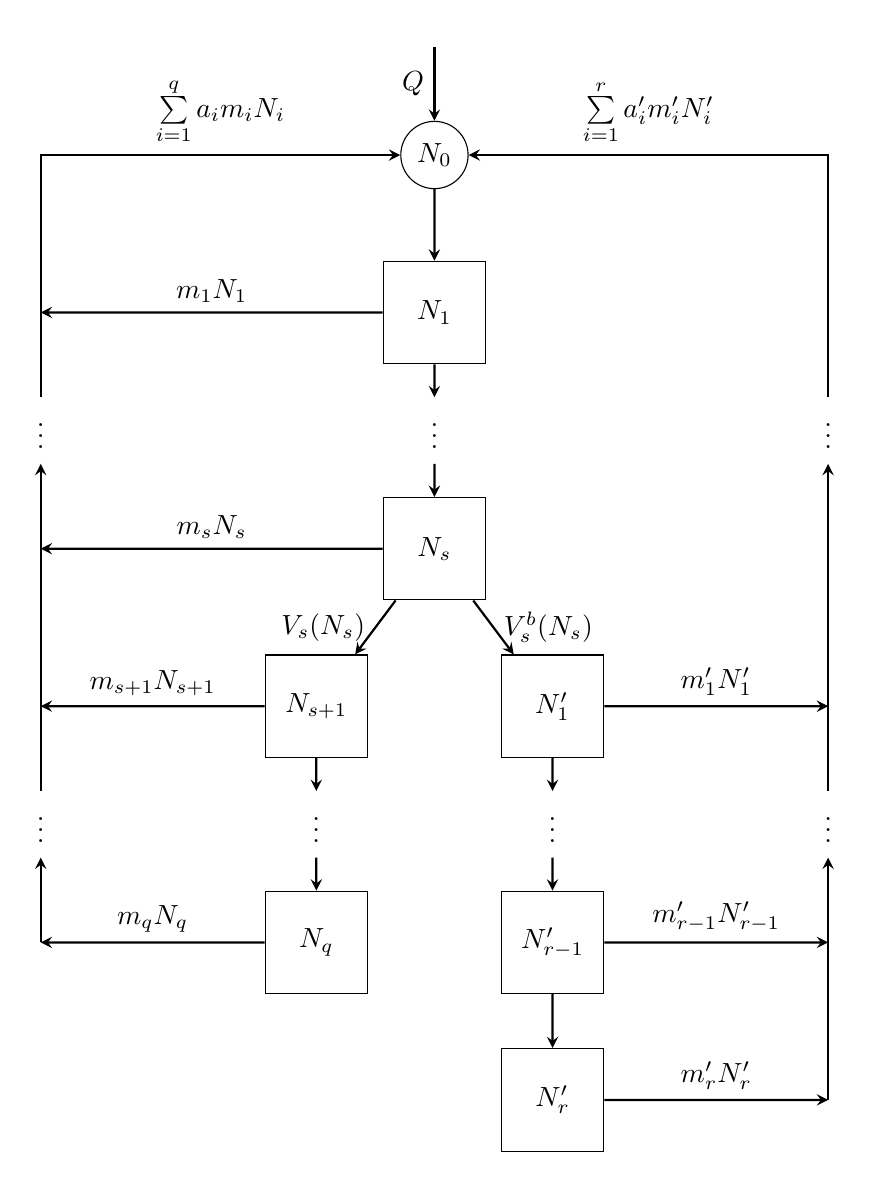
\begin{tikzpicture}

        \usetikzlibrary{shapes.geometric, calc}

        \tikzstyle{roundnode} = [draw, circle, text centered];
        \tikzstyle{squarenode} = [draw, regular polygon, regular polygon sides=4, text centered, inner sep=0, text width=0.92cm];
        \tikzstyle{arrow} = [thick, ->, >=stealth];
        

        \node[roundnode] (N0) at (0,0) {$N_0$};

        \node[squarenode] (N1) at ([yshift=-2cm]N0) {$N_1$};
        \node (ND) at ([yshift=-1.5cm]N1) {$\vdots\vphantom{lp}$};
        \node[squarenode] (NS) at ([yshift=-1.5cm]ND) {$N_s$};


        \node[squarenode] (NS1) at ([xshift=-1.5cm,yshift=-2cm]NS) {$N_{s+1}$};
        \node (NSD) at ([yshift=-1.5cm]NS1) {$\vdots\vphantom{lp}$};
        \node[squarenode] (NQ) at ([yshift=-1.5cm]NSD) {$N_q$};


        \node[squarenode] (M1) at ([xshift=1.5cm,yshift=-2cm]NS) {$N'_{1}$};
        \node (MD) at ([yshift=-1.5cm]M1) {$\vdots\vphantom{lp}$};
        \node[squarenode] (Mm1) at ([yshift=-1.5cm]MD) {$N'_{r-1}$};
        \node[squarenode] (MR) at ([yshift=-2cm]Mm1) {$N'_r$};


        \node (QN0) at ([yshift=1.5cm]N0) {};
        \draw [arrow] (QN0) -- node[anchor=east] {$Q$} (N0);

        
        \draw [arrow] (N0) -- (N1);
        \draw [arrow] (N1) -- (ND);
        \draw [arrow] (ND) -- (NS);
        
        \draw [arrow] (NS) -- node[anchor=east] {$V_s(N_s)$} (NS1);
        \draw [arrow] (NS1) -- (NSD);
        \draw [arrow] (NSD) -- (NQ);

        \draw [arrow] (NS) -- node[anchor=west] {$V^b_s(N_s)$} (M1);
        \draw [arrow] (M1) -- (MD);
        \draw [arrow] (MD) -- (Mm1);
        \draw [arrow] (Mm1) -- (MR);

        \node (DBS) at ([xshift=-5cm]ND) {$\vdots\vphantom{lp}$};
        \node (DBR) at ([xshift=5cm]ND) {$\vdots\vphantom{lp}$};
        \node (DBS2) at ($(DBS)!(NSD)!(DBS)$) {$\vdots\vphantom{lp}$};
        \node (DBR2) at ($(DBR)!(MD)!(DBR)$) {$\vdots\vphantom{lp}$};


        \draw[arrow] ($(DBS)!(NQ)!(DBS)$) -- (DBS2);
        \draw[arrow] (DBS2) -- (DBS);
        \draw[arrow] (DBS) |- node[pos=0.75, anchor=south] {$\textstyle\sum\limits_{i=1}^q a_i m_i N_i$} (N0);


        \draw[arrow] ($(DBR)!(MR)!(DBR)$) -- (DBR2);
        \draw[arrow] (DBR2) -- (DBR);
        \draw[arrow] (DBR) |- node[pos=0.75, anchor=south] {$\textstyle\sum\limits_{i=1}^r a'_i m'_i N'_i$} (N0);


        \draw[arrow] (N1) -- node[anchor=south] {$m_1 N_1$} ($(DBS)!(N1)!(DBS)$);
        \draw[arrow] (NS) -- node[anchor=south] {$m_s N_s$} ($(DBS)!(NS)!(DBS)$);
        \draw[arrow] (NS1) -- node[anchor=south] {$m_{s+1} N_{s+1}$} ($(DBS)!(NS1)!(DBS)$);
        \draw[arrow] (NQ) -- node[anchor=south] {$m_q N_q$} ($(DBS)!(NQ)!(DBS)$);
        

        \draw[arrow] (M1) -- node[anchor=south] {$m'_1 N'_1$} ($(DBR)!(M1)!(DBR)$);
        \draw[arrow] (Mm1) -- node[anchor=south] {$m'_{r-1} N'_{r-1}$} ($(DBR)!(Mm1)!(DBR)$);
        \draw[arrow] (MR) -- node[anchor=south] {$m'_{r} N'_{r}$} ($(DBR)!(MR)!(DBR)$);

    \end{tikzpicture}
    \caption{Схема ветвящейся трофической цепи с двумя ветвями. Виды \(N_i\) -- главная цепь, \(N'_i\) -- боковая.} \label{schema_split}
\end{figure}

По схеме можем построить систему дифференциальных уравнений.
\begin{equation} \label{double_full}
    \begin{split}
        & \frac{d N_0}{dt} = Q - V_0(N_0) N_1 + \sum_{i=1}^q a_i m_i N_i + \sum_{i=1}^r a'_i m'_i N'_i, \\
        & \frac{d N_i}{dt} = -m_i N_i + k_i V_{i-1}(N_{i-1}) N_i - V_i(N_i) N_{i+1}, \quad i=\overline{1,s-1},  \overline{s+1,q}, \\
        & \frac{d N_s}{dt} = -m_s N_s + k_s V_{s-1}(N_{s-1}) N_s - V_s(N_s) N_{s+1} - V_s^b(N_s) N'_1, \\
        & \frac{d N'_1}{dt} = -m'_1 N'_1 + k'_1 V_s^b(N_s) N'_1 - V'_1(N'_1) N'_{2}, \\
        & \frac{d N'_k}{dt} = -m'_k N'_k + k'_k V'_{k-1}(N'_{k-1}) N'_k - V'_k(N'_k) N'_{k+1}, \quad k=\overline{2,r}.
    \end{split}
\end{equation} 
Здесь аналогично \(N_{q+1} \equiv 0, N'_{r+1} \equiv 0\).